\section{Creación de un Issue mediante la interfaz web de GitHub}

Como primera actividad se simuló un problema denominado \textbf{Error en el inicio de sesión}. Este Issue fue creado utilizando la interfaz web de GitHub con el propósito de representar una incidencia que debía ser atendida por otro integrante del equipo.

Durante la creación del Issue se registró el título del problema y una descripción de la situación presentada. Posteriormente el Issue fue asignado al integrante Diego Martínez, quien sería el responsable de analizar y resolver la incidencia.



\begin{figure}[H]
\centering
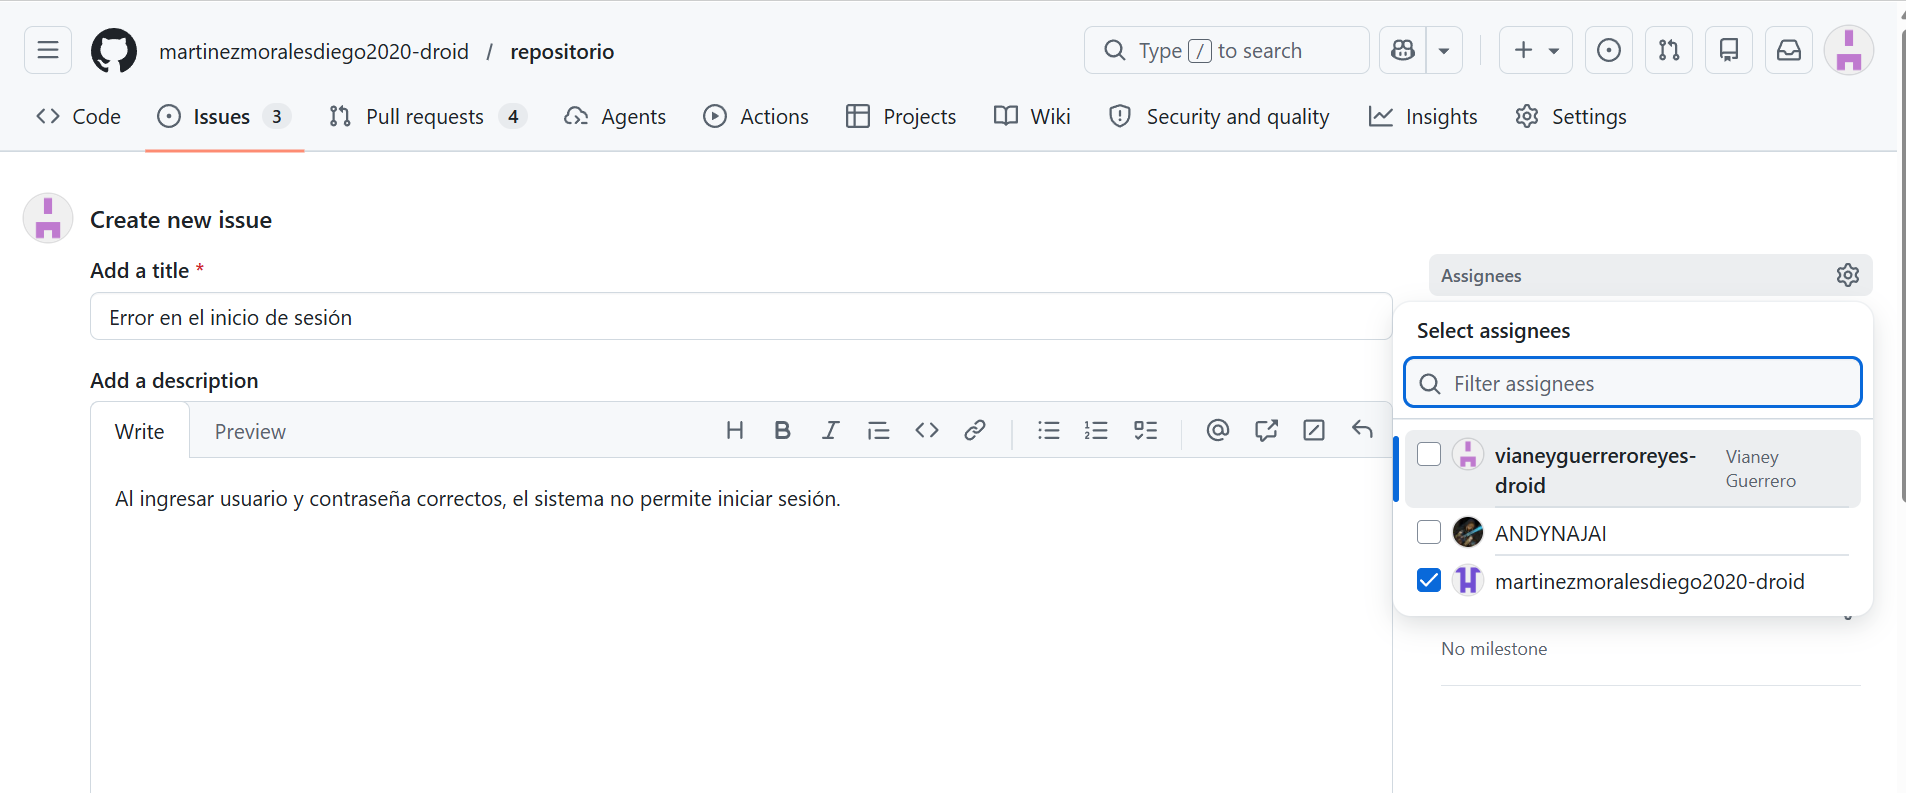
\includegraphics[width=0.9\textwidth]{M1.png}
\caption{Creación del Issue ``Error en el inicio de sesión'' desde GitHub Web.}
\end{figure}

Una vez creado, GitHub registró correctamente la incidencia dentro del repositorio, quedando disponible para su seguimiento y administración.


\begin{figure}[H]
\centering
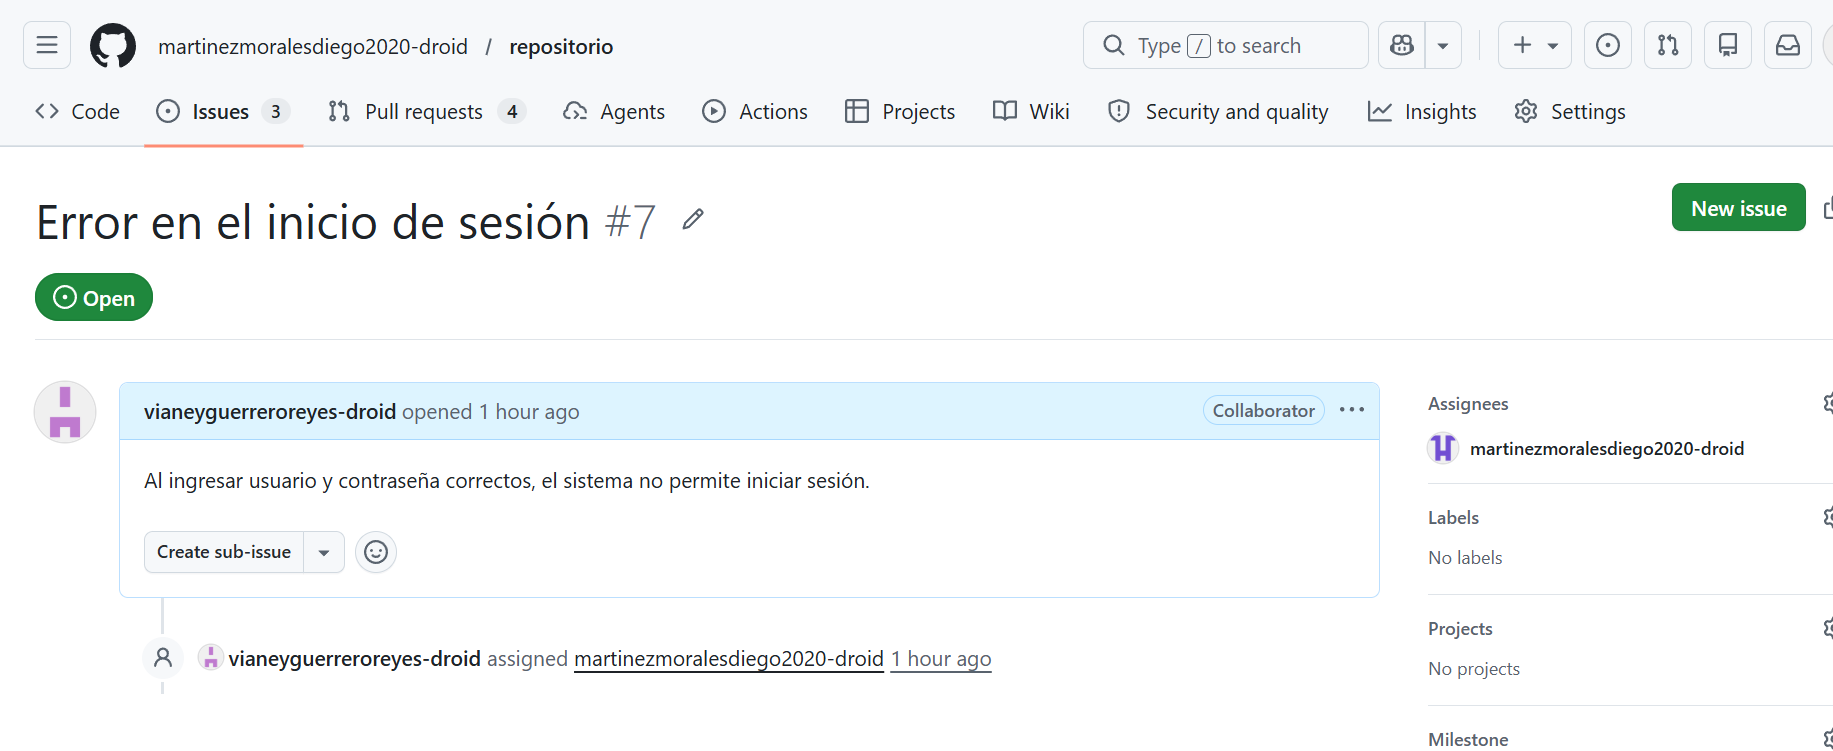
\includegraphics[width=0.9\textwidth]{M2.png}
\caption{Issue ``Error en el inicio de sesión'' registrado en GitHub.}
\end{figure}